\documentclass{ltjsarticle}

\usepackage{luatexja}

\usepackage[haranoaji]{luatexja-preset}
% フォント設定

% 数学パッケージ
\usepackage{amsmath,amssymb,amsthm}
\usepackage{mathtools}

% 図式パッケージ
\usepackage{tikz}
\usetikzlibrary{arrows.meta,positioning,shapes,calc,decorations.pathmorphing}
\usepackage{tikz-cd}

% その他
\usepackage{hyperref}
\usepackage{xcolor}
\usepackage{listings}
\usepackage{tcolorbox}
\tcbuselibrary{listingsutf8,skins,breakable}
\usepackage{booktabs}
\usepackage{enumitem}

% 色定義
\definecolor{catD}{RGB}{70,130,180}
\definecolor{catle}{RGB}{60,179,113}
\definecolor{catlebij}{RGB}{255,165,0}
\definecolor{catwithmin}{RGB}{220,20,60}
\definecolor{leancolor}{RGB}{50,50,50}

% 定理環境
\theoremstyle{definition}
\newtheorem{definition}{定義}[section]
\newtheorem{theorem}[definition]{定理}
\newtheorem{lemma}[definition]{補題}
\newtheorem{proposition}[definition]{命題}
\newtheorem{corollary}[definition]{系}
\newtheorem{example}[definition]{例}
\newtheorem{remark}[definition]{注意}

% Lean コード環境
\lstdefinelanguage{lean}{
  keywords={def,theorem,lemma,structure,where,instance,namespace,end,open,import,variable,example,abbrev,infix,infixr,simp,intro,exact,rfl,by,fun,Type,Prop,let,have,show,refine,apply,cases,with,if,then,else},
  morecomment=[l]{--},
  morecomment=[n]{/-}{-/},
  morestring=[b]",
  sensitive=true,
}

\lstset{
  language=lean,
  basicstyle=\ttfamily\small,
  keywordstyle=\color{blue}\bfseries,
  commentstyle=\color{gray}\itshape,
  stringstyle=\color{orange},
  breaklines=true,
  frame=single,
  backgroundcolor=\color{gray!10},
}

\newtcolorbox{leanbox}[1][]{
  colback=gray!5,
  colframe=gray!50,
  fonttitle=\bfseries,
  title=#1,
  breakable,
}

% タイトル
\title{%
  \Huge 構造塔の圏論的レーン設計\\[0.5em]
  \Large Structure Tower Categorical Lanes:\\
  \large Cat\_D から Cat\_WithMin までの統一的形式化
}
\author{%
  \TeX 文書生成：Claude (Anthropic)\\
  Lean 4 形式化：Codex (OpenAI) 支援\\[1em]
  \small プロジェクト: lean-natural-numbers
}
\date{2025年12月19日}

\begin{document}

\maketitle

\begin{abstract}
本稿では、構造塔（Structure Tower）の圏論的形式化における複数の「レーン」設計について包括的に解説する。
同じ構造塔という対象に対して、射に載せる情報量が異なる複数の圏が存在し、
それらは忘却関手によって階層的に接続される。
最も柔軟な Cat\_D（存在量化による層保存）から、
最も厳格な Cat\_WithMin（minLayer の等式保存）まで、
各レーンの数学的動機、設計原理、および相互関係を明らかにする。
すべての定義と定理は Lean 4 により形式的に検証されている。
\end{abstract}

\tableofcontents
\newpage

%%%%%%%%%%%%%%%%%%%%%%%%%%%%%%%%%%%%%%%%%%%%%%%%%%%%%%%%%%%%%%%%%%%%%%%%%%%%%%%
\section{設計原理と全体像}
%%%%%%%%%%%%%%%%%%%%%%%%%%%%%%%%%%%%%%%%%%%%%%%%%%%%%%%%%%%%%%%%%%%%%%%%%%%%%%%

\subsection{レーン設計の動機}

構造塔理論において、「同じ塔（対象）でも、射に載せる情報量が違う複数の圏がある」
という状況が自然に生じる。これは以下の数学的・応用上の理由による：

\begin{enumerate}[label=(\arabic*)]
  \item \textbf{応用の多様性}：確率論（フィルトレーション）では柔軟な条件が必要だが、
        普遍性の証明では厳格な条件が必要
  \item \textbf{情報の精度}：添字写像 $\phi$ を明示的に持つか、存在のみを保証するか
  \item \textbf{一意性の要求}：minLayer を保存することで射が一意に決まる場合がある
\end{enumerate}

\subsection{主要な圏の階層}

本稿で扱う圏の包含関係を図\ref{fig:main-hierarchy}に示す。

\begin{figure}[htbp]
\centering
\begin{tikzpicture}[
  node distance=2.5cm,
  catnode/.style={rectangle, draw, rounded corners, minimum width=3cm, minimum height=1cm, align=center},
  arrow/.style={-{Stealth}, thick}
]

% ノード配置
\node[catnode, fill=catwithmin!20] (cat2) {\textbf{Cat\_WithMin (Cat2)}\\minLayer 等式保存};
\node[catnode, fill=catlebij!20, below=of cat2] (catlebij) {\textbf{Cat\_LeBij}\\$(map, \phi)$ + 全単射};
\node[catnode, fill=catle!20, below=of catlebij] (catle) {\textbf{Cat\_le}\\$(map, \phi)$ + $\phi$ 単調};
\node[catnode, fill=catle!10, right=3cm of catle] (catleexists) {\textbf{Cat\_le\_exists}\\$\exists$ 単調 $\phi$};
\node[catnode, fill=catD!20, below=of catle] (catd) {\textbf{Cat\_D}\\map のみ + $\exists j$};

% 矢印（忘却関手）
\draw[arrow] (cat2) -- node[right] {\small minLayer を忘却} (catlebij);
\draw[arrow] (catlebij) -- node[right] {\small bijective を忘却} (catle);
\draw[arrow] (catle) -- node[above] {\small $\phi$ をデータ→存在} (catleexists);
\draw[arrow] (catleexists) -- node[right] {\small 単調性を忘却} (catd);
\draw[arrow, dashed] (catle) -- node[left] {\small $\phi$ を忘却} (catd);

% 射の条件ラベル
\node[right=0.5cm of cat2, text=catwithmin] {\footnotesize 最も厳格};
\node[right=0.5cm of catd, text=catD] {\footnotesize 最も柔軟};

\end{tikzpicture}
\caption{構造塔の圏の階層構造。上ほど厳格な条件、下ほど柔軟な条件を持つ。}
\label{fig:main-hierarchy}
\end{figure}

\subsection{射の条件の比較表}

\begin{table}[htbp]
\centering
\caption{各圏における射の条件の比較}
\label{tab:morphism-comparison}
\begin{tabular}{@{}lcccc@{}}
\toprule
\textbf{圏} & \textbf{map} & \textbf{indexMap} & \textbf{層保存} & \textbf{追加条件} \\
\midrule
Cat\_D & $\checkmark$ & $\times$ & $\exists j$ & なし \\
Cat\_le\_exists & $\checkmark$ & $\exists$ 単調 & 明示的 & なし \\
Cat\_le & $\checkmark$ & データ（単調） & 明示的 & なし \\
Cat\_LeBij & $\checkmark$ & データ（単調） & 明示的 & map, $\phi$ 全単射 \\
Cat\_WithMin & $\checkmark$ & データ（単調） & 明示的 & minLayer 等式保存 \\
\bottomrule
\end{tabular}
\end{table}

%%%%%%%%%%%%%%%%%%%%%%%%%%%%%%%%%%%%%%%%%%%%%%%%%%%%%%%%%%%%%%%%%%%%%%%%%%%%%%%
\section{Cat\_D：最小・存在量化のレーン}
\label{sec:cat-d}
%%%%%%%%%%%%%%%%%%%%%%%%%%%%%%%%%%%%%%%%%%%%%%%%%%%%%%%%%%%%%%%%%%%%%%%%%%%%%%%

\subsection{設計思想}

Cat\_D は構造塔の圏の中で最も「薄い」構造を持つ。射は基礎写像 $f: X \to X'$ のみを
持ち、層保存条件は存在量化で表現される。これにより：

\begin{itemize}
  \item より多くの射が存在する（弱い条件）
  \item 確率論における可測写像の自然なモデル化が可能
  \item indexMap の一意性を気にする必要がない
\end{itemize}

\subsection{基本定義}

\begin{definition}[構造塔（minLayer なし）]
構造塔 $T = (X, I, \leq, L)$ は以下のデータからなる：
\begin{itemize}
  \item $X$：台集合（carrier）
  \item $(I, \leq)$：添字集合（前順序集合）
  \item $L: I \to \mathcal{P}(X)$：層関数
  \item 被覆性：$\forall x \in X, \exists i \in I, x \in L(i)$
  \item 単調性：$i \leq j \Rightarrow L(i) \subseteq L(j)$
\end{itemize}
\end{definition}

\begin{definition}[Cat\_D の射（HomD）]
構造塔 $T, T'$ に対して、Cat\_D の射 $f: T \to T'$ は：
\begin{itemize}
  \item $f: T.\mathrm{carrier} \to T'.\mathrm{carrier}$（台集合の写像）
  \item 層保存条件：$\forall i \in T.\mathrm{Index}, \exists j \in T'.\mathrm{Index},$
        $f(L_T(i)) \subseteq L_{T'}(j)$
\end{itemize}
\end{definition}

\begin{figure}[htbp]
\centering
\begin{tikzcd}[row sep=large, column sep=large]
  T.L(i) \arrow[r, "f"] \arrow[d, hook] & T'.L(j) \arrow[d, hook] \\
  T.\mathrm{carrier} \arrow[r, "f"'] & T'.\mathrm{carrier}
\end{tikzcd}
\caption{HomD における層保存：各層 $L(i)$ の像は「どこかの」層 $L(j)$ に含まれる。$j$ は明示的に与えられず、存在のみが保証される。}
\label{fig:homd-layer}
\end{figure}

\subsection{Lean 4 実装}

\begin{leanbox}[Cat\_D の定義]
\begin{lstlisting}
structure StructureTower where
  carrier : Type*
  Index : Type*
  [indexPreorder : Preorder Index]
  layer : Index → Set carrier
  covering : ∀ x : carrier, ∃ i : Index, x ∈ layer i
  monotone : ∀ {i j : Index}, i ≤ j → layer i ⊆ layer j

structure HomD (T T' : TowerD) where
  map : T.carrier → T'.carrier
  map_layer : ∀ i : T.Index, ∃ j : T'.Index,
    Set.image map (T.layer i) ⊆ T'.layer j
\end{lstlisting}
\end{leanbox}

\subsection{なぜ minLayer なしが必要か}

\begin{remark}[応用上の動機]
確率論において、フィルトレーション間の可測写像を考える際：
\begin{itemize}
  \item 事象の像が「どこかの」$\sigma$-代数で可測であればよい（存在量化）
  \item indexMap の明示的な構成は不要（選択の自由度）
  \item 同値な確率空間の異なる表現を許容
\end{itemize}
Cat2（minLayer 保存版）の厳密性は普遍性の証明に有用だが、
応用では過剰な制約となることがある。
\end{remark}

%%%%%%%%%%%%%%%%%%%%%%%%%%%%%%%%%%%%%%%%%%%%%%%%%%%%%%%%%%%%%%%%%%%%%%%%%%%%%%%
\section{Cat\_le：データ版（indexMap を明示的に持つ）}
\label{sec:cat-le}
%%%%%%%%%%%%%%%%%%%%%%%%%%%%%%%%%%%%%%%%%%%%%%%%%%%%%%%%%%%%%%%%%%%%%%%%%%%%%%%

\subsection{設計思想}

Cat\_le では、Cat\_D の射に \textbf{明示的な添字写像 indexMap} を追加する。
この indexMap は単調性を満たす必要がある。

\begin{figure}[htbp]
\centering
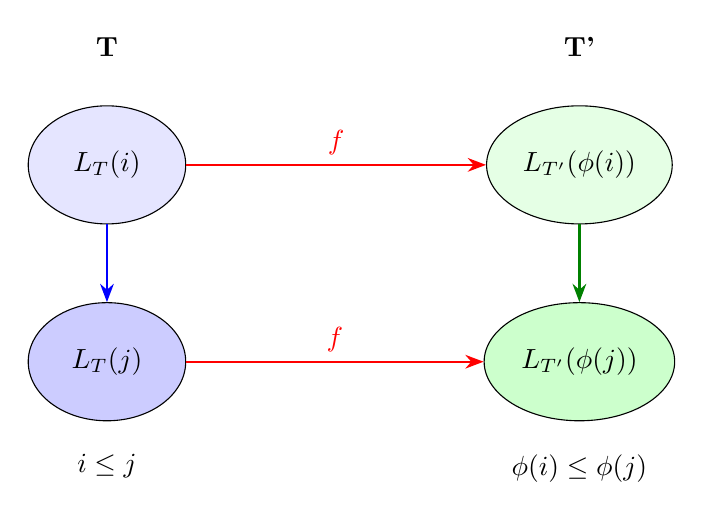
\begin{tikzpicture}[
  node distance=3cm,
  setnode/.style={ellipse, draw, minimum width=2cm, minimum height=1.5cm},
  arrow/.style={-{Stealth}, thick}
]

% 左側（T）
\node[setnode, fill=blue!10] (Ti) at (0,0) {$L_T(i)$};
\node[setnode, fill=blue!20] (Tj) at (0,-2.5) {$L_T(j)$};
\node[below=0.3cm of Tj] {$i \leq j$};
\draw[arrow, blue] (Ti) -- (Tj);

% 右側（T'）
\node[setnode, fill=green!10] (Tpi) at (6,0) {$L_{T'}(\phi(i))$};
\node[setnode, fill=green!20] (Tpj) at (6,-2.5) {$L_{T'}(\phi(j))$};
\node[below=0.3cm of Tpj] {$\phi(i) \leq \phi(j)$};
\draw[arrow, green!50!black] (Tpi) -- (Tpj);

% 水平の射
\draw[arrow, red] (Ti) -- node[above] {$f$} (Tpi);
\draw[arrow, red] (Tj) -- node[above] {$f$} (Tpj);

% ラベル
\node[above=0.5cm of Ti] {\textbf{T}};
\node[above=0.5cm of Tpi] {\textbf{T'}};

\end{tikzpicture}
\caption{HomLe における層保存：$\phi$ が順序を保存し、$f$ が層を $\phi$ で指定された層に送る。}
\label{fig:homle-layer}
\end{figure}

\subsection{基本定義}

\begin{definition}[Cat\_le の射（HomLe）]
構造塔 $T, T'$ に対して、Cat\_le の射 $(f, \phi): T \to T'$ は：
\begin{itemize}
  \item $f: T.\mathrm{carrier} \to T'.\mathrm{carrier}$（基礎写像）
  \item $\phi: T.\mathrm{Index} \to T'.\mathrm{Index}$（添字写像）
  \item $\phi$ は単調：$i \leq j \Rightarrow \phi(i) \leq \phi(j)$
  \item 層構造の保存：$x \in L_T(i) \Rightarrow f(x) \in L_{T'}(\phi(i))$
\end{itemize}
\end{definition}

\begin{remark}[Cat\_D との差分]
Cat\_D では「$\exists j$ such that $f(L(i)) \subseteq L(j)$」という条件だったが、
Cat\_le では「$j = \phi(i)$」と明示的に indexMap で指定される。
これにより射の等式が $(f, \phi)$ の両方の等式で決まる。
\end{remark}

\subsection{Lean 4 実装}

\begin{leanbox}[Cat\_le の定義]
\begin{lstlisting}
structure HomLe (T T' : TowerD) where
  map : T.carrier → T'.carrier
  indexMap : T.Index → T'.Index
  indexMap_mono : Monotone indexMap
  layer_preserving : ∀ (i : T.Index) (x : T.carrier),
    x ∈ T.layer i → map x ∈ T'.layer (indexMap i)
\end{lstlisting}
\end{leanbox}

\subsection{具体例：自然数の構造塔}

\begin{example}[後者関数による射]
自然数の構造塔 $\mathrm{natTowerD}$ において、層を $L(n) = \{k \in \mathbb{N} \mid k \leq n\}$ と定義する。
後者関数 $\mathrm{succ}: \mathbb{N} \to \mathbb{N}$ は Cat\_le の自己射を与える：
\begin{itemize}
  \item $\mathrm{map} = \mathrm{succ}$
  \item $\mathrm{indexMap} = \mathrm{succ}$（層番号を1つずらす）
  \item 層保存：$k \leq i \Rightarrow k+1 \leq i+1$
\end{itemize}
\end{example}

%%%%%%%%%%%%%%%%%%%%%%%%%%%%%%%%%%%%%%%%%%%%%%%%%%%%%%%%%%%%%%%%%%%%%%%%%%%%%%%
\section{Cat\_le\_exists：indexMap を「存在」に落とす}
\label{sec:cat-le-exists}
%%%%%%%%%%%%%%%%%%%%%%%%%%%%%%%%%%%%%%%%%%%%%%%%%%%%%%%%%%%%%%%%%%%%%%%%%%%%%%%

\subsection{設計動機}

Cat\_le（データ版）では、同じ $f$ に対して異なる indexMap $\phi_1, \phi_2$ を持つ
射 $(f, \phi_1)$ と $(f, \phi_2)$ が異なる射として扱われる。
これは忘却関手を Cat\_D へ定義する際に問題となる。

Cat\_le\_exists では、indexMap をデータとして保持せず、
「単調な indexMap が存在する」という条件のみを要求する。

\begin{definition}[HomLeExists]
構造塔 $T, T'$ に対して、Cat\_le\_exists の射は：
\begin{align*}
\{ f: T.\mathrm{carrier} \to T'.\mathrm{carrier} \mid 
&\exists \phi: T.\mathrm{Index} \to T'.\mathrm{Index}, \\
&\quad \phi \text{ は単調} \land \forall i, x, (x \in L_T(i) \Rightarrow f(x) \in L_{T'}(\phi(i))) \}
\end{align*}
\end{definition}

\subsection{Category インスタンスの衝突回避}

Lean では同じ型に複数の Category インスタンスを定義すると衝突が起きる。
このため、Cat\_le\_exists では \textbf{ラッパー型} \texttt{TowerD\_LeExists} を導入する。

\begin{leanbox}[ラッパー型の定義]
\begin{lstlisting}
structure TowerD_LeExists where
  toTowerD : TowerD

instance : Coe TowerD_LeExists TowerD := ⟨TowerD_LeExists.toTowerD⟩
\end{lstlisting}
\end{leanbox}

%%%%%%%%%%%%%%%%%%%%%%%%%%%%%%%%%%%%%%%%%%%%%%%%%%%%%%%%%%%%%%%%%%%%%%%%%%%%%%%
\section{Forgetful Functors（Data $\to$ Exists $\to$ D）}
\label{sec:functors}
%%%%%%%%%%%%%%%%%%%%%%%%%%%%%%%%%%%%%%%%%%%%%%%%%%%%%%%%%%%%%%%%%%%%%%%%%%%%%%%

\subsection{忘却関手の全体像}

各レーン間の接続は忘却関手によって与えられる。

\begin{figure}[htbp]
\centering
\begin{tikzcd}[row sep=large, column sep=huge]
  \texttt{TowerD} \arrow[r, "\texttt{forgetIndexMap}"] \arrow[dr, "\texttt{forgetLeToD}"', bend right=15] 
  & \texttt{TowerD\_LeExists} \arrow[d, "\texttt{forgetToD}"] \\
  & \texttt{TowerD\_D}
\end{tikzcd}
\caption{忘却関手の可換図式。forgetLeToD = forgetIndexMap $\circ$ forgetToD。}
\label{fig:forgetful-functors}
\end{figure}

\subsection{各関手の定義}

\begin{definition}[forgetIndexMap]
データ版 Cat\_le（TowerD 上）から存在版 Cat\_le\_exists（TowerD\_LeExists 上）への関手。
indexMap のデータを忘れ、存在証明として保持する。
\end{definition}

\begin{definition}[forgetToD]
Cat\_le\_exists から Cat\_D への関手。
単調な indexMap の存在を用いて、層保存の存在量化条件を満たす。
\end{definition}

\begin{theorem}[forgetToD の faithfulness]
関手 $\texttt{forgetToD}: \texttt{TowerD\_LeExists} \to \texttt{TowerD\_D}$ は faithful である。
\end{theorem}

\begin{proof}
射の等式は map の等式に帰着するため、異なる射が同じ像を持つことはない。
\end{proof}

\subsection{Lean 4 実装}

\begin{leanbox}[forgetToD の faithful 性]
\begin{lstlisting}
instance : Functor.Faithful forgetToD where
  map_injective := by
    intro T T' f g h
    have hm : (forgetToD.map f).map = (forgetToD.map g).map := by
      exact congrArg (fun k => k.map) h
    apply TowerD_LeExists.HomLeExists.ext
    intro x
    exact congrArg (fun m => m x) hm
\end{lstlisting}
\end{leanbox}

%%%%%%%%%%%%%%%%%%%%%%%%%%%%%%%%%%%%%%%%%%%%%%%%%%%%%%%%%%%%%%%%%%%%%%%%%%%%%%%
\section{Cat\_LeBij：全単射条件付きレーン}
\label{sec:cat-lebij}
%%%%%%%%%%%%%%%%%%%%%%%%%%%%%%%%%%%%%%%%%%%%%%%%%%%%%%%%%%%%%%%%%%%%%%%%%%%%%%%

\subsection{設計動機}

Cat\_LeBij は Cat\_le に「map と indexMap が全単射」という条件を追加したレーンである。
これは「台集合の取り換え（全単射）」を伴う変換を扱う際に有用である。

\begin{tcolorbox}[colback=red!5,colframe=red!50!black,title=重要な注意]
\textbf{bijective + layer-preserving でも、逆写像が layer-preserving とは限らない。}

したがって、Cat\_LeBij は Cat\_le における同型射の groupoid では\textbf{ない}。
単なる「bijective lane」である。
\end{tcolorbox}

\subsection{定義}

\begin{definition}[HomLeBij]
Cat\_LeBij の射は、HomLe の射 $(f, \phi)$ であって：
\begin{itemize}
  \item $f: T.\mathrm{carrier} \to T'.\mathrm{carrier}$ が全単射
  \item $\phi: T.\mathrm{Index} \to T'.\mathrm{Index}$ が全単射
\end{itemize}
を満たすもの。
\end{definition}

\begin{figure}[htbp]
\centering
\begin{tikzpicture}[
  node distance=2cm,
  setnode/.style={rectangle, draw, rounded corners, minimum width=2.5cm, minimum height=1.2cm, align=center}
]

% 左側
\node[setnode, fill=blue!10] (X) at (0,0) {$X$};
\node[setnode, fill=blue!10] (I) at (0,-2.5) {$I$};

% 右側
\node[setnode, fill=green!10] (Xp) at (5,0) {$X'$};
\node[setnode, fill=green!10] (Ip) at (5,-2.5) {$I'$};

% 矢印
\draw[-{Stealth}, thick, red] (X) -- node[above] {$f$ (全単射)} (Xp);
\draw[-{Stealth}, thick, orange] (I) -- node[above] {$\phi$ (全単射)} (Ip);

% ラベル
\node[left=0.3cm of X] {carrier};
\node[left=0.3cm of I] {Index};

\end{tikzpicture}
\caption{HomLeBij の構造：carrier と Index の両方で全単射。}
\label{fig:homlebij}
\end{figure}

\subsection{逆写像が層保存しない例}

\begin{example}[groupoid でない理由]
以下の状況を考える：
\begin{itemize}
  \item $T$：層 $L_T(0) = \{a\}, L_T(1) = \{a, b\}$
  \item $T'$：層 $L_{T'}(0) = \{x, y\}, L_{T'}(1) = \{x, y\}$（早く安定）
  \item $f(a) = x, f(b) = y$（全単射）
  \item $\phi(0) = 0, \phi(1) = 1$（恒等、全単射）
\end{itemize}
このとき、$f$ は層を保存するが、$f^{-1}$ は保存しない：
$y \in L_{T'}(0)$ だが $f^{-1}(y) = b \notin L_T(0)$。
\end{example}

%%%%%%%%%%%%%%%%%%%%%%%%%%%%%%%%%%%%%%%%%%%%%%%%%%%%%%%%%%%%%%%%%%%%%%%%%%%%%%%
\section{Cat\_TowerD\_Bij：安定した命名}
\label{sec:cat-towerd-bij}
%%%%%%%%%%%%%%%%%%%%%%%%%%%%%%%%%%%%%%%%%%%%%%%%%%%%%%%%%%%%%%%%%%%%%%%%%%%%%%%

\subsection{命名の整理}

歴史的に、TowerD 上の bijective レーンは \texttt{Cat\_eq} という名前で呼ばれていた。
しかし、これは minLayer 等式保存のレーン（後述の Cat\_WithMin）と混同されやすい。

そこで：
\begin{itemize}
  \item \texttt{Cat\_TowerD\_Bij}：TowerD 上の bijective レーンの安定名
  \item 実装は \texttt{Cat\_LeBij} に委譲（thin re-export）
\end{itemize}

\begin{leanbox}[Cat\_TowerD\_Bij の定義（re-export）]
\begin{lstlisting}
abbrev TowerD_Bij := TowerD_LeBij

namespace TowerD
abbrev HomBij (T T' : TowerD) : Type := HomLeBij T T'
end TowerD
\end{lstlisting}
\end{leanbox}

%%%%%%%%%%%%%%%%%%%%%%%%%%%%%%%%%%%%%%%%%%%%%%%%%%%%%%%%%%%%%%%%%%%%%%%%%%%%%%%
\section{Cat\_WithMin (Cat2)：minLayer 付きの最も厳格なレーン}
\label{sec:cat-withmin}
%%%%%%%%%%%%%%%%%%%%%%%%%%%%%%%%%%%%%%%%%%%%%%%%%%%%%%%%%%%%%%%%%%%%%%%%%%%%%%%

\subsection{設計思想}

Cat\_WithMin（または Cat2）は、対象に \textbf{minLayer 関数}を持たせ、
射が minLayer を\textbf{等式で}保存することを要求する最も厳格なレーンである。

この厳格さにより：
\begin{itemize}
  \item 射の一意性が保証される
  \item 普遍性（自由構造塔など）の証明が可能になる
  \item indexMap が minLayer から完全に決定される
\end{itemize}

\subsection{基本定義}

\begin{definition}[StructureTowerWithMin]
minLayer を持つ構造塔 $T = (X, I, \leq, L, \ell)$ は、構造塔に加えて：
\begin{itemize}
  \item $\ell: X \to I$（minLayer 関数）
  \item $\forall x, x \in L(\ell(x))$（minLayer は実際に $x$ を含む）
  \item $\forall x, i, (x \in L(i) \Rightarrow \ell(x) \leq i)$（minLayer は最小）
\end{itemize}
\end{definition}

\begin{definition}[homeq（minLayer 等式保存の射）]
構造塔 $T, T'$（minLayer 付き）に対して、homeq の射 $(f, \phi): T \to T'$ は：
\begin{itemize}
  \item HomLe のすべての条件に加えて
  \item \textbf{minLayer 保存}：$\ell_{T'}(f(x)) = \phi(\ell_T(x))$
\end{itemize}
\end{definition}

\begin{figure}[htbp]
\centering
\begin{tikzcd}[row sep=large, column sep=large]
  X \arrow[r, "f"] \arrow[d, "\ell_T"'] & X' \arrow[d, "\ell_{T'}"] \\
  I \arrow[r, "\phi"'] & I'
\end{tikzcd}
\caption{homeq における可換図式：minLayer が等式で保存される。}
\label{fig:homeq-commute}
\end{figure}

\subsection{minLayer 保存の重要性}

\begin{theorem}[射の一意性]
自由構造塔からの射において、minLayer 保存条件により indexMap $\phi$ が一意に決定される。
\end{theorem}

\begin{proof}[証明の概略]
任意の射 $\Psi: F(X) \to T$ で $\Psi.\mathrm{map} = f$ を満たすものに対して：
\begin{align*}
\Psi.\mathrm{indexMap}(x) &= \Psi.\mathrm{indexMap}(\ell_{F(X)}(x)) \\
&= \ell_T(\Psi.\mathrm{map}(x)) \quad \text{(minLayer 保存)} \\
&= \ell_T(f(x))
\end{align*}
したがって、$\Psi.\mathrm{indexMap}$ は完全に決定される。
\end{proof}

\subsection{Lean 4 実装}

\begin{leanbox}[Cat\_WithMin の定義]
\begin{lstlisting}
structure StructureTowerWithMin where
  carrier : Type u
  Index : Type v
  [indexPreorder : Preorder Index]
  layer : Index → Set carrier
  covering : ∀ x : carrier, ∃ i : Index, x ∈ layer i
  monotone : ∀ {i j : Index}, i ≤ j → layer i ⊆ layer j
  minLayer : carrier → Index
  minLayer_mem : ∀ x, x ∈ layer (minLayer x)
  minLayer_minimal : ∀ x i, x ∈ layer i → minLayer x ≤ i

structure Hom (T T' : StructureTowerWithMin) where
  map : T.carrier → T'.carrier
  indexMap : T.Index → T'.Index
  indexMap_mono : ∀ {i j}, i ≤ j → indexMap i ≤ indexMap j
  layer_preserving : ∀ (i : T.Index) (x : T.carrier),
    x ∈ T.layer i → map x ∈ T'.layer (indexMap i)
  minLayer_preserving : ∀ x, T'.minLayer (map x) = indexMap (T.minLayer x)
\end{lstlisting}
\end{leanbox}

%%%%%%%%%%%%%%%%%%%%%%%%%%%%%%%%%%%%%%%%%%%%%%%%%%%%%%%%%%%%%%%%%%%%%%%%%%%%%%%
\section{Cat\_eq：WithMin レーンの入口}
\label{sec:cat-eq}
%%%%%%%%%%%%%%%%%%%%%%%%%%%%%%%%%%%%%%%%%%%%%%%%%%%%%%%%%%%%%%%%%%%%%%%%%%%%%%%

\subsection{命名の整理}

\texttt{Cat\_eq} は minLayer 等式保存レーンへの入口として固定されるモジュールである。
実装は \texttt{Cat\_WithMin} に委譲され、これはさらに \texttt{CAT2\_complete} を re-export する。

\begin{leanbox}[Cat\_eq の定義]
\begin{lstlisting}
import MyProjects.ST.CAT.Cat_WithMin

/-!
# Cat_eq: the `minLayer`-equality lane

This module name is kept as a convenient entry point for the lane where 
structure towers carry a chosen `minLayer` and morphisms preserve it 
**by equality** (your `homeq` intuition).
-/
\end{lstlisting}
\end{leanbox}

\subsection{混同を避けるための注意}

\begin{remark}[命名史の整理]
\begin{itemize}
  \item 旧 \texttt{Cat\_eq}（TowerD bijective）$\to$ \texttt{Cat\_TowerD\_Bij} へ移動
  \item 現 \texttt{Cat\_eq} = minLayer 等式保存（WithMin レーン）
  \item bijective レーンが必要な場合は \texttt{Cat\_LeBij} を使用
\end{itemize}
\end{remark}

%%%%%%%%%%%%%%%%%%%%%%%%%%%%%%%%%%%%%%%%%%%%%%%%%%%%%%%%%%%%%%%%%%%%%%%%%%%%%%%
\section{まとめと展望}
%%%%%%%%%%%%%%%%%%%%%%%%%%%%%%%%%%%%%%%%%%%%%%%%%%%%%%%%%%%%%%%%%%%%%%%%%%%%%%%

\subsection{本稿の成果}

\begin{enumerate}
  \item \textbf{レーン設計の全体像}を明確化：Cat\_D から Cat\_WithMin までの階層構造
  \item \textbf{各レーンの数学的動機}を解説：応用に応じた条件の選択
  \item \textbf{忘却関手による接続}を整理：Data $\to$ Exists $\to$ D
  \item \textbf{命名の整理}：Cat\_eq の意味を明確化
\end{enumerate}

\subsection{レーン選択の指針}

\begin{table}[htbp]
\centering
\caption{応用に応じたレーン選択}
\begin{tabular}{@{}ll@{}}
\toprule
\textbf{応用} & \textbf{推奨レーン} \\
\midrule
確率論の可測写像 & Cat\_D \\
フィルトレーションの時刻保存 & Cat\_le \\
普遍性の証明 & Cat\_WithMin \\
台集合の同型的変換 & Cat\_LeBij \\
\bottomrule
\end{tabular}
\end{table}

\subsection{今後の展望}

\begin{itemize}
  \item 極限・余極限の存在と構成
  \item 随伴関手の完全証明
  \item 確率論（フィルトレーション、停止時間）への応用の深化
  \item 連続時間への拡張
\end{itemize}

%%%%%%%%%%%%%%%%%%%%%%%%%%%%%%%%%%%%%%%%%%%%%%%%%%%%%%%%%%%%%%%%%%%%%%%%%%%%%%%
\appendix
\section{型ラッパ一覧}
%%%%%%%%%%%%%%%%%%%%%%%%%%%%%%%%%%%%%%%%%%%%%%%%%%%%%%%%%%%%%%%%%%%%%%%%%%%%%%%

Lean では Category インスタンスの衝突を避けるため、以下のラッパ型を使用する：

\begin{table}[htbp]
\centering
\caption{型ラッパと対応するレーン}
\begin{tabular}{@{}lll@{}}
\toprule
\textbf{ラッパ型} & \textbf{射の型} & \textbf{レーン} \\
\midrule
\texttt{TowerD} & \texttt{HomLe} & Cat\_le（data） \\
\texttt{TowerD\_LeExists} & \texttt{HomLeExists} & Cat\_le\_exists \\
\texttt{TowerD\_D} & \texttt{HomD} & Cat\_D \\
\texttt{TowerD\_LeBij} & \texttt{HomLeBij} & Cat\_LeBij \\
\texttt{StructureTowerWithMin} & \texttt{Hom} & Cat\_WithMin \\
\bottomrule
\end{tabular}
\end{table}

%%%%%%%%%%%%%%%%%%%%%%%%%%%%%%%%%%%%%%%%%%%%%%%%%%%%%%%%%%%%%%%%%%%%%%%%%%%%%%%
\section{Sanity Check 集}
%%%%%%%%%%%%%%%%%%%%%%%%%%%%%%%%%%%%%%%%%%%%%%%%%%%%%%%%%%%%%%%%%%%%%%%%%%%%%%%

以下の等式は \texttt{rfl} で証明できる sanity check である：

\begin{leanbox}[Sanity checks]
\begin{lstlisting}
-- Cat_le: 恒等射は恒等関数
example (T : TowerD) (x : T.carrier) : (𝟙 T : T ⟶ T).map x = x := rfl

-- Cat_le: 合成は関数合成
example (T T' T'' : TowerD) (f : T ⟶ T') (g : T' ⟶ T'') :
    (f ≫ g).map = g.map ∘ f.map := rfl

-- forgetLeToD: 恒等射の保存
example (T : TowerD) (x : T.carrier) :
    (forgetLeToD.map (𝟙 T)).map x = x := rfl

-- Cat_WithMin: 合成の定義
example (T T' T'' : TowerWithMin) (f : T ⟶ T') (g : T' ⟶ T'') :
    (f ≫ g).map = g.map ∘ f.map := rfl
\end{lstlisting}
\end{leanbox}

%%%%%%%%%%%%%%%%%%%%%%%%%%%%%%%%%%%%%%%%%%%%%%%%%%%%%%%%%%%%%%%%%%%%%%%%%%%%%%%
\section*{参考文献}
%%%%%%%%%%%%%%%%%%%%%%%%%%%%%%%%%%%%%%%%%%%%%%%%%%%%%%%%%%%%%%%%%%%%%%%%%%%%%%%

\begin{enumerate}
  \item Bourbaki, N. \textit{Éléments de mathématique: Théorie des ensembles}. Hermann.
  \item Mac Lane, S. \textit{Categories for the Working Mathematician}. 2nd ed., Springer, 1998.
  \item Awodey, S. \textit{Category Theory}. 2nd ed., Oxford University Press, 2010.
  \item The mathlib Community. \textit{The Lean Mathematical Library}. \url{https://github.com/leanprover-community/mathlib4}
  \item Williams, D. \textit{Probability with Martingales}. Cambridge University Press, 1991.
\end{enumerate}

\end{document}
